\documentclass[12pt]{article}
\usepackage[utf8]{inputenc}
\usepackage{amsmath,amssymb,hyperref,array,xcolor,multicol,verbatim,mathpazo}
\usepackage[normalem]{ulem}
\usepackage[pdftex]{graphicx}
\usepackage{parskip}
\usepackage{authblk}

\begin{document}

\title{STAT4710 Data Science and Analytics using Python}
\author{Ng Tze Kean}
\affil{Student No.: 721370290002}
\date{27 Feb 2024}
\maketitle

\newpage

\section*{Question 1}
\subsection*{a}

\begin{center}
    $B = \begin{bmatrix}
            2 & 2 & 2  \\
            5 & 8 & 0  \\
            0 & 2 & 3  \\
            0 & 0 & 10
        \end{bmatrix}$
\end{center}

\subsection*{b}

\begin{center}
    $A = \begin{bmatrix}
            2 & 1 & 0 & 0  \\
            1 & 1 & 1 & 1  \\
            0 & 0 & 0 & 10 \\
        \end{bmatrix}$
\end{center}

\subsection*{c}
\begin{center}
    $
        \begin{alignedat}{2}
            AB \vec{v_2}    & = \vec{x} \\
            \begin{bmatrix}
                9 & 12 & 4   \\
                7 & 12 & 15  \\
                0 & 0  & 100
            \end{bmatrix}
            \cdot \vec{v_2} & =
            \begin{bmatrix}
                80 \\
                80 \\
                100
            \end{bmatrix}
        \end{alignedat}
    $
\end{center}
Solving for $\vec{v_2}$ using matrix row reduction
\begin{center}
    $
        \begin{array}{ccc|c}
            9 & 12 & 4   & 80  \\
            7 & 12 & 15  & 80  \\
            0 & 0  & 100 & 100
        \end{array}
        \sim\hspace{1em}
        \begin{array}{ccc|c}
            6 & 9  & 1  & 40 \\
            7 & 12 & 15 & 80 \\
            0 & 0  & 1  & 1
        \end{array}
        \sim \hspace{1em}
        \begin{array}{ccc|c}
            6 & 9  & 1  & 40 \\
            7 & 12 & 15 & 80 \\
            0 & 0  & 1  & 1
        \end{array}
        \sim\newline
        \begin{array}{ccc|c}
            9 & 0  & 0  & 99/2 \\
            7 & 12 & 15 & 53   \\
            0 & 0  & 1  & 1
        \end{array}
        \sim\hspace{1em}
        \begin{array}{ccc|c}
            1 & 0 & 0 & 11/2  \\
            0 & 1 & 0 & 53/24 \\
            0 & 0 & 1 & 1
        \end{array}
    $

    $
        \vec{v_2} =
        \begin{bmatrix}
            11/2 \\
            53/24   \\
            1
        \end{bmatrix}
    $
\end{center}

\newpage

\section*{Problem 2}

\subsection*{a}
\begin{center}
    $
        \begin{alignedat}{2}
            \sigma(-x) & =\frac{1}{1+e^x}           \\
                       & = \frac{1}{e^{x-x}+e^x}    \\
                       & = \frac{1}{e^x(1+e^{-x})}  \\
                       & = \frac{e^x}{1+e^{-x}}     \\
                       & = \frac{e^x-1+1}{1+e^{-x}} \\
                       & = 1 - \sigma(x)
        \end{alignedat}
    $
\end{center}

\subsection*{b}
\begin{center}
    $
        \begin{alignedat}{1}
            \frac{d }{dx} \sigma(x) & = (1+e^{-x})^{-1}                           \\
                                    & = (1+e^{-x})^{-2}(e^{-x})(-1)               \\
                                    & = \frac{e^{-x}}{(1+e^{-x})^{2}}             \\
                                    & = (1+e^{-x})^{-1} \frac{e^{-x}}{(1+e^{-x})} \\
                                    & = \sigma (x) (1-\sigma(x))
        \end{alignedat}
    $
\end{center}

\newpage

\subsection*{c}
where the red line represents the $\sigma(x)$, and green line $\frac{d }{dx} \sigma(x)$

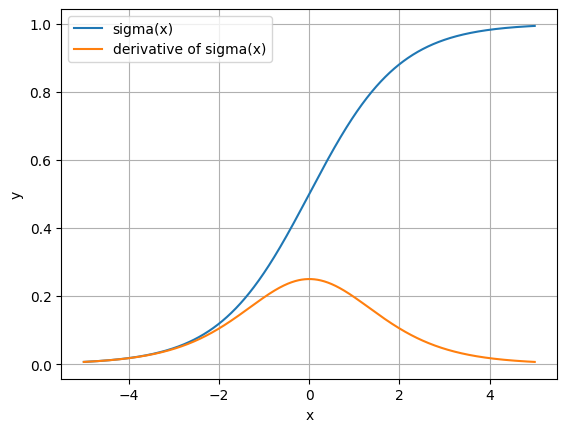
\includegraphics[width=\textwidth]{question2.png}

\newpage

\section*{Problem 3}

\begin{center}
    $
        \begin{alignedat}{2}
            f(c)                 & = \frac{1}{n} \sum_{i=1}^{n} (x_i - c)^2                                   \\
                                 & = \frac{1}{n} \sum_{i=1}^{n} (x_i^2 -2x_i c + c^2)                         \\
                                 & = \frac{1}{n} \sum_{i=1}^{n} x_i^2 - \frac{2c}{n} \sum_{i=1}^{n} x_i + c^2 \\
            \parbox{3in}{To find c which minimises f(c),}                                                     \\                                                                    \\
            \frac{d }{dc} f(c)   & = - \frac{2}{n} \sum_{i=1}^{n} x_i + 2c                                    \\
            c                    & = \frac{1}{n} \sum_{i=1}^{n}(x_i)                                          \\
            \parbox{3in}{To prove that it is the mininum, we check the 2nd derivative}                        \\
            \frac{d2 }{dc2} f(c) & = 2
        \end{alignedat}
    $
\end{center}

Since the 2nd derivative is positive, then the turning point computed
must be a minimum point

\newpage

\section*{Question 4}

Given the following,
\begin{center}
    $
        \begin{alignedat}{1}
            P (C)      & = 0.01  \\
            P (Pos|C)  & = 0.8   \\
            P (Pos|'C) & = 0.096 \\
        \end{alignedat}
    $
\end{center}

Solve for $P(C|Pos)$

\begin{center}
    $
        \begin{alignedat}{1}
            P(C|Pos) & = \frac{P (Pos|C) P (C)}{P (Pos)}\\
                     & =\frac{P (Pos|C) P (C)}{P (Pos|C) P (C) + P (Pos|`C) P (`C)}\\
                     & =\frac{0.8 \times0.01}{0.8 \times0.01 + 0.096 \times0.99} \\
                     & =0.0776
        \end{alignedat}
    $
\end{center}

\newpage

\section*{Problem 5}

Since the distribution is approximately normal with $n \geq 30$, we can
use the fact that the area under a normal distribution within 1SD
from mean is $68\%$ and 2SD is $95\%$. Then, based on the graph, 2SD is
likely to be $12+$. Working backwards, 1SD can be approximated to be $6.1$.
\\\\
Answer: b

\newpage

\section*{Problem 6}

\subsection*{a}
From the lecture slides, we can obtain the following information,\\
Population = Entire population of America (45million)\\
Sample = 10million

\subsection*{b}

Null hypothesis is 43\% vote for Roosevelt.\\
Alternate hypothesis is that Roosevelt should be getting more votes\\

$H_0: \mu=0.43$

$H_{A}: \mu>0.43$

\subsection*{c}

\[
    Z = \frac{\bar{x} - \mu_0}{\frac{\sigma}{\sqrt{n}}}
\]

For a significance level of 1\%, the critical value is 2.326 for a right tail
test.

\[
    \sigma = \frac{\bar{x} - \mu_0}{Z} \times \sqrt{n}
\]

We can reorder the formula and find that when n is large at 10million, the
standard deviation is huge, but when n is smaller at 100, then the
standard deviation is small at 0.86 making the sample more likely to be
a chance error.

\end{document}